% set 0 inch indentation
\setlength{\parindent}{0in} 
% set paragraph space = 1 space
\setlength{\parskip}{1em}
% set line space 1.5
\setlength{\baselineskip}{1.6em}

\chapter{PRELIMINARY EXPERIMENTS}
\label{ch:results}


\section{Experimental Setup}
\paragraph{}
To collect the raw data, experiments are performed in the living room of my house in Bangkok, Thailand, which was built from reinforced concrete with tile, as shown in Figure \ref{fig:home}. The system can detect vibration in a range around 3 meters, and this room has dimension 3.5 $\times$ 3.5 $\text{m}^2$. The hardware should be installed near the corner in order to be as suitable for the application as possible.

\begin{figure}[H]
  \centering
  \caption[Living room area used for preliminary experiment.]{\emph{Living room area used for preliminary experiment.}}\label{fig:home}
  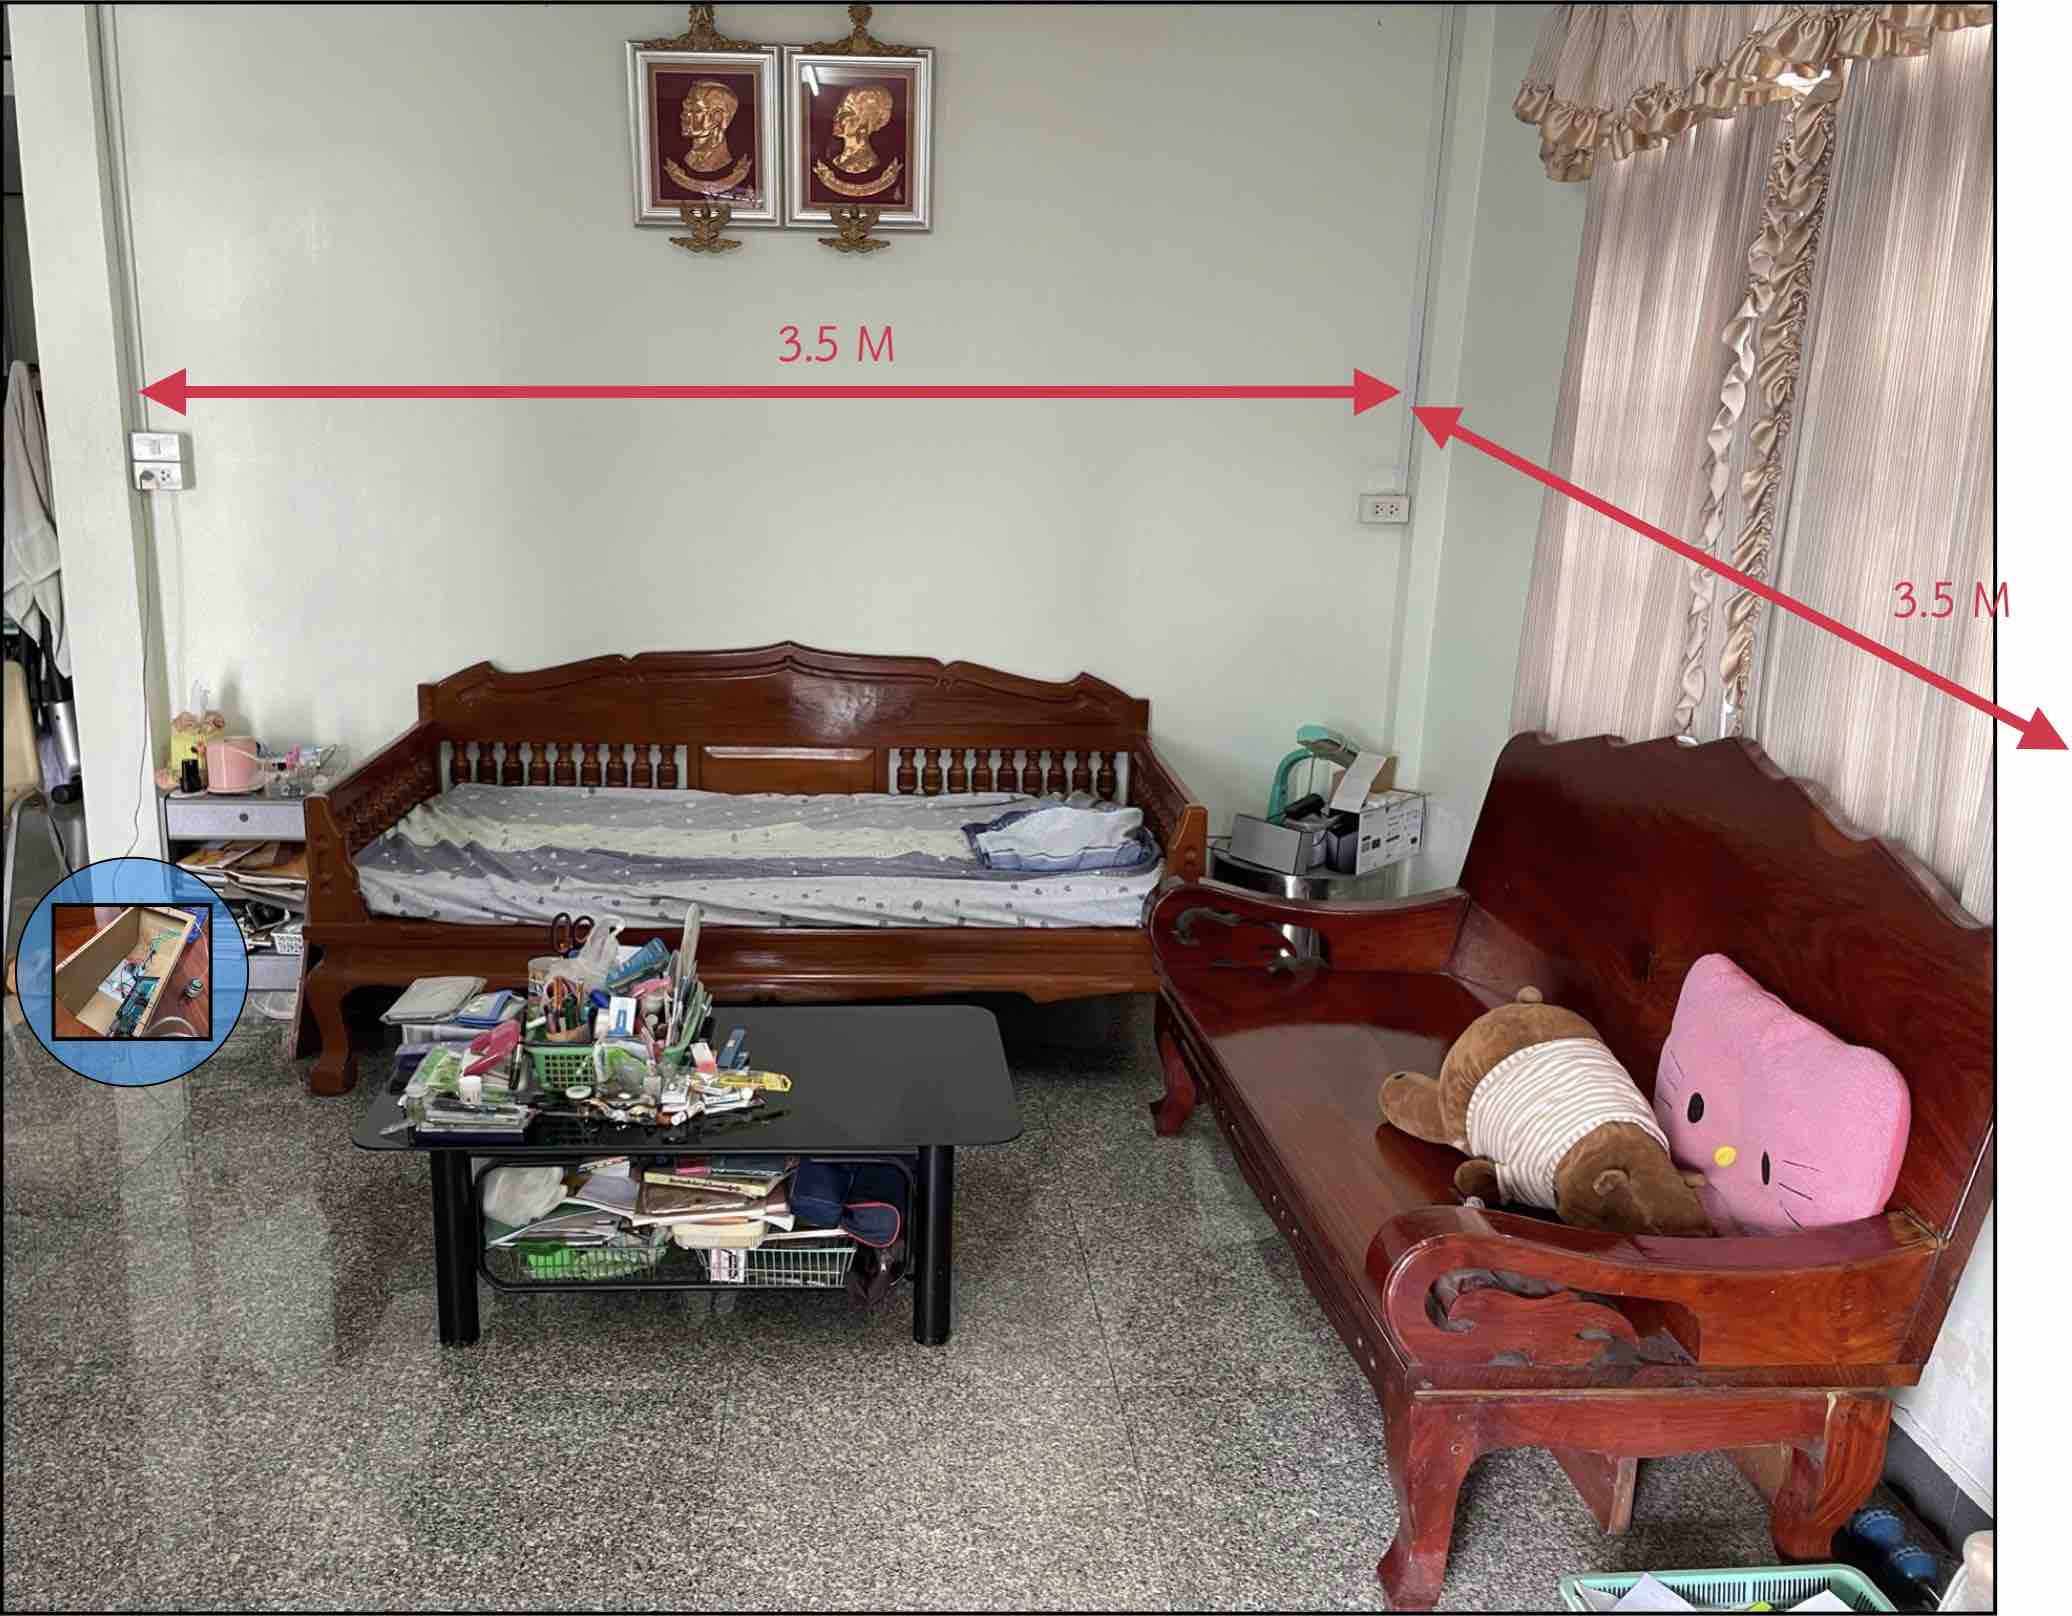
\includegraphics[scale = 0.15]{figures/home.jpg}  
\end{figure}

\section{Ordinary Activiting}
\paragraph{}
There are several activities that occur normally during daily life. I focus on typical activities such as walking, sitting, standing and lying down, as shown in Table \ref{tab:number_action}. Under COVID-19, I cannot invite outside volunteers to come indoor for data collection. However, if the COVID situation in Thailand improves, I will invite approximate 3-5 friends to participate in ordinary activities. In the meantime, I plan to collect activities of four subjects, my father, my mother, my older brother, and me. Details of them are shown in Table \ref{tab:participants}.

\begin{table}[H]
\begin{center}
\caption[The detail of each activity and its number of action.]{\emph{The detail of each activity and its number of action.} \\ \hspace{\textwidth}}\label{tab:number_action}
\begin{tabular}{ l r }
  \textbf{Human Activity} & \textbf{Number of action}\\
\hline
Walking & 2,500 \\
\hline
Sitting & 400 \\
\hline
Standing & 400 \\
\hline
Lying & 400 \\
\hline
   \end{tabular}
\end{center}
 \end{table}
 
\begin{table}[H]
\begin{center}
\caption[Details on each participant.
]{\emph{Details on each participant.} 
\\ \hspace{\textwidth}}\label{tab:participants}
\begin{tabular}{c c c c}
  \textbf{Subject} & \textbf{Sex} &  \textbf{Age} & \textbf{Weight $(kg)$}  \\
\hline

1 & M & 23  & 58 \\
\hline

2 & M & 25  & 70 \\
\hline

3 & M & 55  & 70 \\
\hline

4 & F & 58  & 75 \\
\hline

   \end{tabular}
\end{center}
 \end{table}
  
\section{Deployment}
\paragraph{}
The desirable system should be plug \& play. Therefore, every component such as seismic sensor, embedded system and Raspberry Pi must be integrated into a small box requiring only a power adapter, as shown in Figure \ref{fig:application}. When anomaly activities occur, an alert message should be sent via the LINE application to me. I plan to train on data from the living room and test on the dining room in my house, as shown in \ref{fig:dining}.

\begin{figure}[H]
  \centering
  \caption[The complete application.]{\emph{The complete system.}} \label{fig:application}
  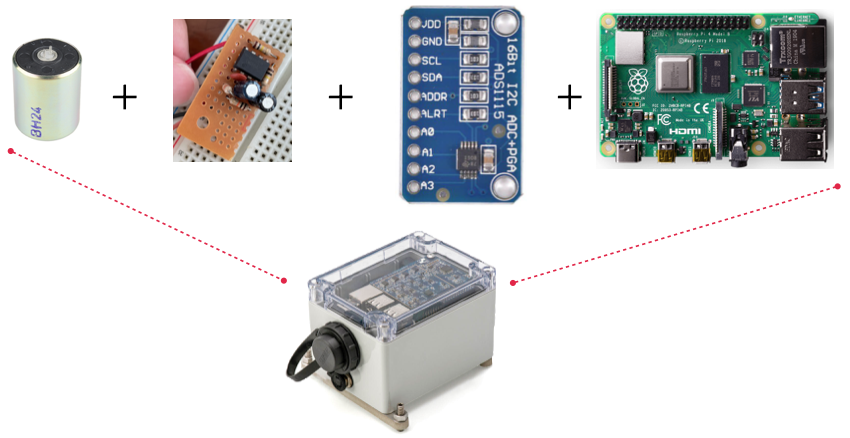
\includegraphics[scale = 0.35]{figures/application.png}  
\end{figure}

\begin{figure}[H]
  \centering
  \caption[The dining room in my home.]{\emph{The dining room in my home.}} \label{fig:dining}
  \includegraphics[scale = 0.07]{figures/dining.jpg}  
\end{figure}

\FloatBarrier